\section{Markt und Preise}

\subsection{Wirtschaftskreislauf}
\begin{multicols}{2}
	\subsubsection{Einfach}
	\includegraphics[width=9cm]{images/einfachWS.jpg}
	\subsubsection{Erweitert}
	\includegraphics[width=9cm]{images/erweiterWS.jpg}
\end{multicols}
\subsubsection{Märkte}
\includegraphics[width=15cm]{images/markte.png}

\subsection{Knappheitssituation}
\begin{itemize}
	\item[\-] Die volkswirtschaftliche Ausgangslage
	\begin{itemize}
		\item Unbeschränkte Bedürfnisse stehen knappe Ressourcen gegenüber
	\end{itemize}
	\item[\-] Notwendige Entscheidungen in dieser Knappheitssituation
	\begin{itemize}
		\item Wie wird das verfügbare (Zeit/Finanz-)Budget auf unterschiedliche Verwendungszwecke aufgeteilt?
	\end{itemize}
	\item[\-] Die Konsequenz: \textbf{Opportunitätskosten}
	\begin{itemize}
		\item Kosten, die bei einer Entscheidung anfallen, dass die Vorteile einer Handlungsalternative nicht realisiert werden können (z.B. Lohnverzicht während Studium)
		\item Die Opportunitätskosten zeigen die Knappheit von Gütern in Form von Preisen an
	\end{itemize}
	\item[\-] Es gibt zwei unterschiedliche Vorstellungen, wie eine Volkswirtschaft organisiert sein muss, damit knappe Ressourcen effizient genutzt werden können:
	\begin{itemize}
		\item \textbf{Planwirtschaft}
		\subitem Ressourcen gehören Staat
		\subitem Staat lenkt Ressourceneinsatz
		\item \textbf{Marktwirtschaft}
		\subitem Ressourcen gehören privaten Haushalten und Firmen 
		\subitem Private Haushalte/Firmen entscheiden über Ressourceneinsatz
		\subitem Preis spielt Hauptrolle
	\end{itemize}
\end{itemize}

\subsection{Mikroökonomisches Grundmodell}
Vorgesetzt wird das \textbf{Modell der vollkommenen Konkurrenz:}
\begin{itemize}
	\item Das Gut ist homogen
	\item Es gibt eine grosse Anzahl von Anbietern und Nachfragern
	\item Keine Marktzutrittshemmnisse
	\item Anbieter und Nachfrager sind über Mengen und Preise vollständig informiert
\end{itemize}
$\rightarrow$ Nur der Preis spielt eine Rolle, Dinge wie Qualität, Image, usw. nicht!\\

\begin{multicols}{2}
	\subsubsection{Konsumentenrente}
	Zahlungsbereitschaft des Käufers für ein Gut,
	abzüglich des Preises, den er tatsächlich dafür bezahlen muss\\
	\includegraphics[width=7cm]{images/kr.jpg}
	\subsubsection{Produzentenrente}
	Erlös des Verkäufers für ein Gut, abzüglich der
	Kosten, die ihm für Erwerb oder Herstellung des Gutes entstanden sind\\
	\includegraphics[width=7cm]{images/pr.jpg}
\end{multicols}

\subsubsection{Wohlfahrt}
Gesamte Rente, die auf einem Markt entsteht (Summe
aus Konsumenten- und Produzentenrente)\\
\begin{figure*}[h]
	\centering
	\includegraphics[width=6cm]{images/wohlfahrt.jpg}
\end{figure*}
\centering
\fcolorbox{red}{white}{Rente = Geschenk, für das man nichts bezahlen muss}
\flushleft
\clearpage
\pagebreak

\subsection{(Staatliche) Preiseingriffe}
\begin{multicols}{2}
	\subsubsection{Höchstpreis}
	\includegraphics[width=7cm]{images/hochstpreis.jpg}
	Wohlfahrtsverlust (rote Fläche), zum künstlich tief gehaltenen Preis entsteht Überschussnachfrage (Nachfrage > Angebot)
	\columnbreak
	\subsubsection{Mindestpreis}
	\includegraphics[width=7cm]{images/mindestpreis.jpg}
	Wohlfahrtsverlust (rote Fläche), zum künstlich hoch gehaltenen Preis entsteht Überschussangebot (Angebot > Nachfrage)
\end{multicols}

\subsection{Elastizität}

\subsubsection{Preiselastizität der Nachfrage}
\begin{multicols}{2}
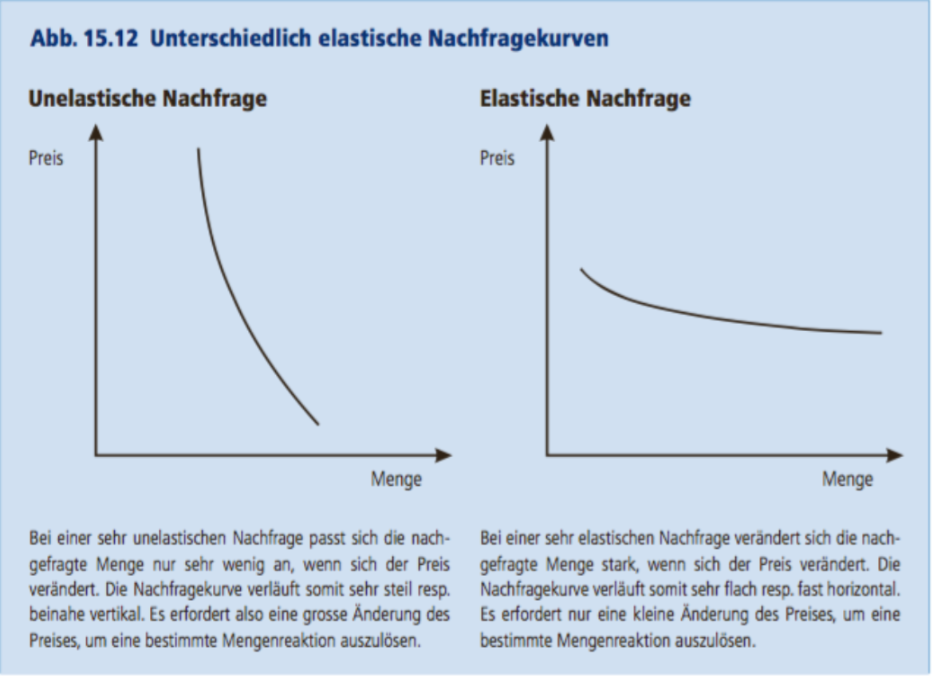
\includegraphics[width=\linewidth]{images/elastischeNachfrage.png}
\columnbreak
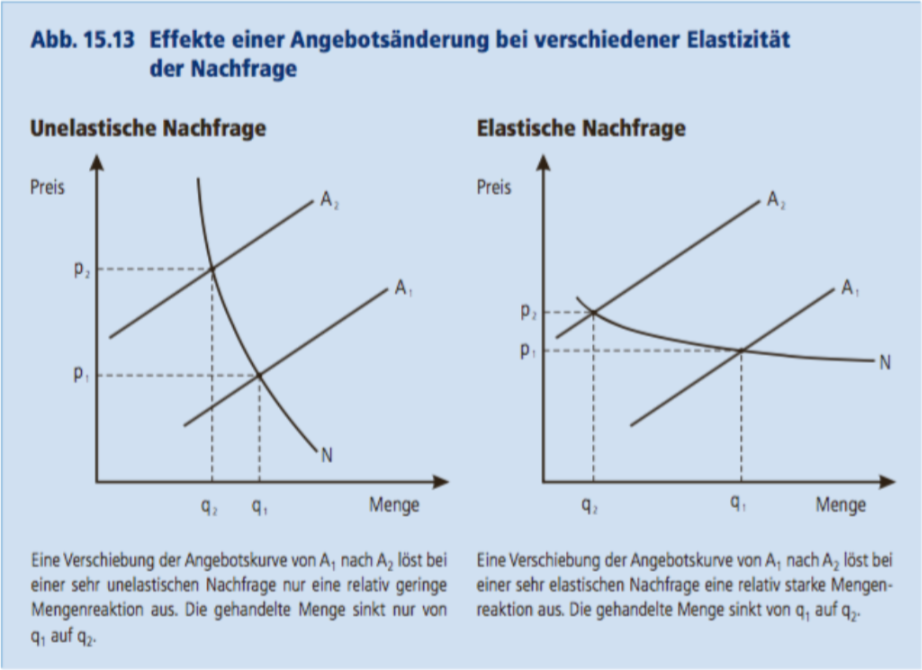
\includegraphics[width=\linewidth]{images/elastischeNachfrage2.png}
\end{multicols}
\begin{minipage}{0.7\linewidth}
	$\textnormal{Preiselastizität der Nachfrage} = \dfrac{\textnormal{Veränderung der nachefragten Menge in \%}}{\textnormal{Veränderung des Preises in \%}}$\\
	\vspace{\baselineskip}
	Die Preiselastizität der Nachfrage ist umso geringer (unelastisch), desto
	\begin{itemize}
		\item weniger Substitutionsmöglichkeiten es gibt.
		\item wichtiger und lebensnotwendiger das Gut ist.
		\item geringer der Anteil der Ausgaben für dieses Gut ist.
		\item kurzfristiger der Effekt betrachtet wird.
	\end{itemize}
	\vfill\null
\end{minipage}%
\hspace{0.04\linewidth}
\begin{minipage}{0.25\linewidth}
	Beispiele für die Preiselastizität der Nachfrage
	\begin{itemize}
		\item{\makebox[2.2cm]{Erbsen\hfill}} 2.8
		\item{\makebox[2.2cm]{Juwelen\hfill}} 2.6
		\item{\makebox[2.2cm]{Kalbfleisch\hfill}} 1.6
		\item{\makebox[2.2cm]{Kino\hfill}} 0.9
		\item{\makebox[2.2cm]{Opern\hfill}} 0.2
		\item{\makebox[2.2cm]{Salz\hfill}} 0.1
	\end{itemize}
\end{minipage}
\clearpage

\subsubsection{Preiselastizität des Angebots}
$\textnormal{Preiselastizität des Angebots} = \dfrac{\textnormal{Veränderung der angebotenen Menge in \%}}{\textnormal{Veränderung des Preises in \%}}$\\
\vspace{\baselineskip}
Die Preiselastizität des Angebots ist umso geringer (unelastisch), desto
\begin{itemize}
	\item weniger haltbar und lagerfähig ein Gut ist.
	\item weniger rasch das Gut in beliebiger Menge hergestellt werden kann.
	\item kurzfristiger der Effekt betrachtet wird.
\end{itemize}

\subsubsection{Einkommenselastizität}
$\textnormal{Einkommenselastizität} = \dfrac{\textnormal{Veränderung der nachgefragten Menge in \%}}{\textnormal{Veränderung des Einkommens in \%}}$\\
\vspace{\baselineskip}
Vier Fälle können hier unterschieden werden:
\begin{itemize}
	\item Einkommenselastizität gleich null
	\item Einkommenselastizität zwischen null und eins
	\item Einkommenselastizität grösser als eins
	\item Einkommenselastizität kleiner als null
\end{itemize}

\subsection{Beitrag des Staates für eine funktionierende Marktwirtschaft}
Bereitstellung eines Rechtssystems, das Eigentumsrechte und Vertragsrechte klar definiert und durchsetzt.
\begin{itemize}
	\item Eigentumsrechte und Vertragsrechte.
\end{itemize}
Korrigierender Eingriff des Staates bei Marktversagen.
\begin{itemize}
	\item Falls frei gebildete Preise falsche relative Knappheiten anzeigen oder Akteure daran gehindert werden, auf Preissignale zu reagieren (Monopolmacht, externe Effekte, öffentliche Güter).
\end{itemize}
Ausgestaltung politisch gewünschter Regulierungen ohne grössere Beeinträchtigung der wirtschaftlichen Effizienz.
\begin{itemize}
	\item Eingriffe in die Marktwirtschaft so gestalten, dass ein Ziel durch eine bestimmte Regulierung mit möglichst geringer Beeinträchtigung der Effizienz und damit des Wohlstandes erreicht werden kann (Regulierungsabschätzung).
\end{itemize}

\subsubsection{Regulierungsfolgenabschätzung RFA}
\textbf{Was sind die Kostenfolgen von Gesetzesvorlagen?}\\
Wie lassen sie sich verlässlich prognostisch abschätzen? Die sogenannte RFA soll noch vor der Einsetzung und Durchführung einer Gesetzesvorlage deren Wirkungen auf die Schweizer Wirtschaft sowie insbesondere kleinere und mittlere Unternehmen einschätzen. Die Eidgenössische Finanzkontrolle (EFK) hat diesbezüglich beträchtliche Mängel identifiziert: Eine Mehrheit der bundesrätlichen Botschaften zu Gesetzesvorlagen erfüllt die Anforderungen bezüglich Abschätzung ihrer Folgen nicht. Es sind denn auch Stimmen laut geworden, welche die Schaffung einer unabhängigen Kontrollstelle für Regulierungsfolgen vorschlagen. Ist das sinnvoll?\\
\textbf{Defizite}\\
Verschiedene Studien haben in den Jahren nach der Einführung der RFA gezeigt, dass ihre Ergebnisse nur selten und sehr begrenzt Einfluss auf die Meinungsbildung und Entscheidung im Gesetzgebungsprozess haben. Die Parlamentarische Verwaltungskontrolle hielt schon 2005 fest, dass die Qualität der RFA zudem oft zu wünschen übrig lässt, weil viele Bundesämter keine Erfahrungen mit ökonomischen Analysen hätten.\\
Um diesen Defiziten entgegenzuwirken, wurde 2006 mit der vertieften RFA eine ergänzende Massnahme eingeführt, welche bei Gesetzesprojekten mit besonders starken Auswirkungen auf die Wirtschaft zum Einsatz kommen soll. Erste Auswertungen bescheinigten dieser Form der RFA tatsächlich eine qualitative Verbesserung gegenüber dem regulären Abschätzungsverfahren. Die Studie der EFK kommt nun aber zum Schluss, dass auch in Fällen, in denen eine vertiefte RFA hätte durchgeführt werden müssen, aus Ressourcengründen darauf verzichtet wurde.\\
\textbf{Wie soll das Problem gelöst werden?}
Das Problem wird in der Qualität des Informationsangebots gesehen, ohne zu fragen: Wer soll das lesen? Parlamentarier jeder Couleur beklagen nun wieder einmal lauthals, wie falsch sie informiert worden sind. Interessant wäre indes zu erfahren, wer von ihnen überhaupt schon einmal eine RFA gelesen hat. Es dürften wenige sein. Dies liegt unter anderem daran, dass eine RFA eine trockene Lektüre und sowohl für die Macher als auch für die Leser unattraktiv ist.\\
\vspace{\baselineskip}
\small{NZZ, 13. Februar 2017}

\clearpage
\pagebreak